\def\ktitle{IDE ASSIGNMENT}
\def\kauthor{Koushik Kalyani}
\def\kcontact{koushikkalyani369@gmail.com}
\def\kmodule{IITH - Future Wireless Communication}
%\renewcommand{\thesection}{\arabic{section}}
%\renewcommand{\thesubsection}{\arabic{subsection}}
%\titleformat{\subsubsection}{\normalfont\itshape\filcenter}{\thesubsubsection}{1em}{}
\documentclass[journal,12pt,twocolumn]{IEEEtran}
\usepackage{enumitem}
%\renewcommand{\thesection}{\arabic{section}}
%\renewcommand{\thesubsection}{\arabic{subsection}}
\usepackage{tikz}
\usepackage{circuitikz}
\usepackage{karnaugh-map}
\usepackage{tabularx}
\usepackage{circuitikz}
\usepackage{tikz}
\usepackage{titlesec}
\title{\ktitle}
\author{\kauthor\\\kcontact\\\kmodule}
\begin{document}
\maketitle
\tableofcontents
\section{\textbf{Question}}
$A=a_1a_0$ and $B=b_1b_0$ are two 2-bit unsigned binary numbers. If $F(a_1,a_0,b_1,b_0)$ is a Boolean function such that $F = 1$ only when $A>B$, and $F=0$ otherwise, then $F$ can be minimized to the form \rule{9mm}{0.4pt}
\begin{enumerate}[label=(\Alph*)]
	\item $a_1\bar b_1+a_1a_0\bar b_0$
	\item $a_1\bar b_1+a_1a_0\bar b_0+a_0\bar b_0\bar b_1$
	\item $a_1a_0\bar b_0 + a_0\bar b_0\bar b_1$
	\item $a_1\bar b_1+a_1a_0\bar b_0 + a_0\bar b_0b_1$  
\end{enumerate}

\section{\textbf{Answer}}
The above question can be solved by using Truth Table and karnaugh-map.\\
\subsection{\centering Truth Table}
\begin{tabularx}{0.45\textwidth}{
	| >{\centering\arraybackslash}X
	| >{\centering\arraybackslash}X
	| >{\centering\arraybackslash}X
	| >{\centering\arraybackslash}X
	| >{\centering\arraybackslash}X|
	}\hline
	\textbf{$a_1$}&\textbf{$a_0$}&\textbf{$b_1$}&\textbf{$b_0$}&\textbf{$F$}\\
	\hline
	0&0&0&0&0\\
	\hline
	0&0&0&1&0\\
	\hline
        0&0&1&0&0\\
	\hline
	0&0&1&1&0\\
	\hline
	0&1&0&0&1\\
	\hline
	0&1&0&1&0\\
	\hline
	0&1&1&0&0\\
	\hline
	0&1&1&1&0\\
	\hline
        1&0&0&0&1\\
	\hline
	1&0&0&1&1\\
	\hline
	1&0&1&0&0\\
	\hline
	1&0&1&1&0\\
	\hline
	1&1&0&0&1\\
	\hline
	1&1&0&1&1\\
	\hline
	1&1&1&0&1\\
	\hline
	1&1&1&1&0\\
	\hline
\end{tabularx}
\begin{center} 
 Truth table for Boolean funtion $F$
\end{center}
\subsection{\centering K-Map Implentation}
\resizebox{0.45\textwidth}{!}{%
	\begin{karnaugh-map}[4][4][1][$b_1b_0$][$a_1a_0$]
		\maxterms{1,2,3,5,6,7,10,0,11,15}
		\minterms{4,12,13,8,9,14}
		\implicant{12}{9}
		\implicant{4}{12}
		\implicantedge{12}{12}{14}{14}
	\end{karnaugh-map}%
}
\begin{center}
Fig. 1\\
\end{center}
Therefore, the Boolean function is $F=a_1\bar b_1+a_1a_0\bar b_0+a_0\bar b_0\bar b_1$.\\
\section{\textbf{Logic Diagram}}
\resizebox{0.5\textwidth}{!}{
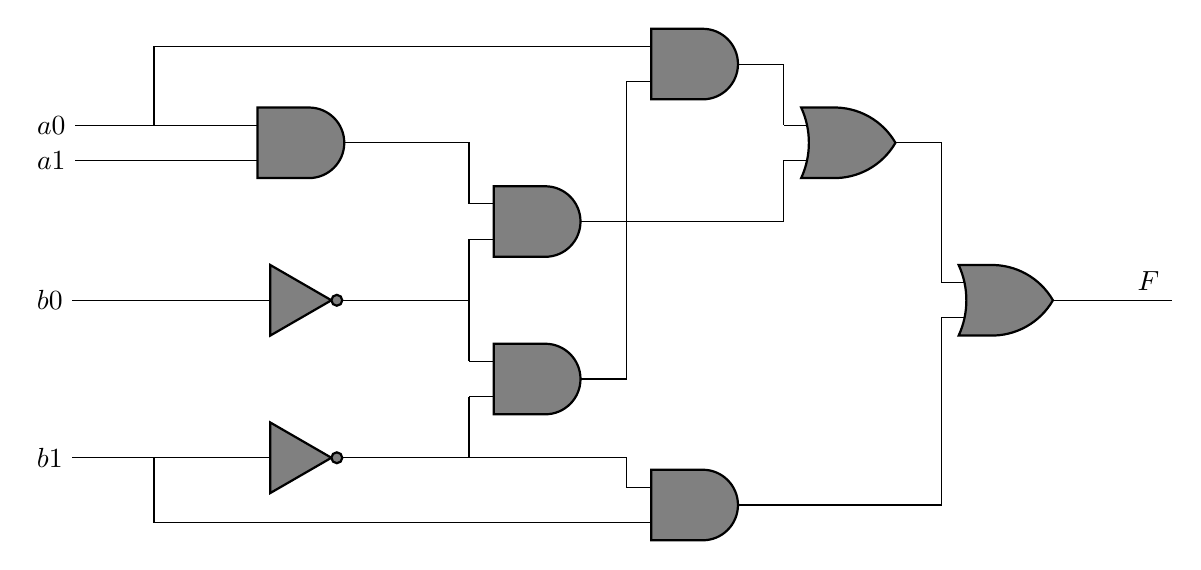
\begin{tikzpicture}
	\ctikzset{
		logic ports=ieee,
		logic ports/scale=0.8,
		logic ports/fill=gray}
	\node[and port](a) at (2,-2){};
	\node[not port](b0) at (2,-4){};
	\node[not port](b1) at (2,-6){};
	\node[and port](c) at (5,-3){};
	\node[and port](d) at (5,-5){};
	\node[and port](b) at (7,-1){};
	\node[and port](e) at (7,-6.6){};
        \node[or port](f) at (9,-2){};
	\node[or port](g) at (11,-4){};
	\draw(a.out)-|(c.in 1);
	\draw(b0.out)-|(c.in 2);
	\draw(b0.out)-|(d.in 1);
	\draw(b1.out)-|(d.in 2);
	\draw(d.out)-|(b.in 2);
	\draw(f.out)-|(g.in 1);
	\draw(e.out)-|(g.in 2);
	\draw(c.out)-|(f.in 2);
	\draw(b.out)-|(f.in 1);
	\draw(b1.out)-|(e.in 1);
	\draw(a.in 1)-- ++(-2,0) node[left]{$a0$};
	\draw(a.in 2)-- ++(-2,0) node[left]{$a1$};
	\draw(b0.in)-- ++(-2.2,0) node[left]{$b0$};
	\draw(b1.in)-- ++(-2.2,0) node[left]{$b1$};
	\draw(b.in 1)-| ++(-6,-1);
	\draw(e.in 2)-| ++(-6,0.82);
	\draw(g.out)-- ++(1.2,0) node[near end,above]{$F$};
\end{tikzpicture}
}
\begin{center}
	Fig. 2
\end{center}
	\section{\textbf{Components}}
	\begin{tabularx}{0.45\textwidth}{
			| >{\centering\arraybackslash}X
			| >{\centering\arraybackslash}X
			| >{\centering\arraybackslash}X |
			}
			\hline
			\textbf{Components}&\textbf{Values}&\textbf{Quantity}\\
			\hline
			Arduino & Uno & 1\\
			\hline
			Jumper Wires & M-M & 6\\
			\hline
			Breadboard & & 1\\
			\hline
	\end{tabularx}
\section{\textbf{Implementation}}
\begin{tabularx}{0.45\textwidth}{
		| >{\centering\arraybackslash}X
		| >{\centering\arraybackslash}X
		| >{\centering\arraybackslash}X|}
\hline
	\textbf{Arduino PIN}&\textbf{INPUT}&\textbf{OUTPUT}\\
	\hline
	2&$a_1$& \\
	\hline
	4&$a_0$&\\
	\hline
	6&$b_1$&\\
	\hline
	8&$b_0$&\\
	\hline
	13&&$F$\\
	\hline

\end{tabularx}\\
\\
\centering
Connections\\
\textbf{Procedure}
\begin{enumerate}[label={\arabic*}.]
	\item Connect the circuit as per the above table.
	\item Connect inputs to Vcc for Logic 1, ground for Logic 0.
	\item Execute the circuit using the below codes.\\
		\vspace{\baselineskip}
		\textit{Approach 1}\\
                \begin{tabularx}{0.45\textwidth}{
				| >{\centering\arraybackslash}X|}
			\hline
                           https://github.com/koushikkalyani/FWC/blob\\/main/IDE/IDE.cpp\\
			\hline
		\end{tabularx}\\
		\vspace{\baselineskip}
		\textit{Approach 2}\\
		\begin{tabularx}{0.45\textwidth}{| >{\centering\arraybackslash}X|}
			\hline
			https://github.com/koushikkalyani/FWC/blob\\/main/IDE/IDE2.cpp\\
			\hline
		\end{tabularx}\\
		\vspace{\baselineskip}
	\item Change the values of $a_0,a_1,b_0,b_1$ in the Hardware and verify the Truth Table.
\end{enumerate}
\end{document}
